\usemintedstyle{tango}
\setminted[python]{fontsize=\footnotesize, breaklines}
%\setminted[scala]{fontsize=\footnotesize, breaklines}
In the first part of this thesis, we have established a theoretical foundation for multigrid methods, formal languages, and evolutionary program synthesis.
In Chapter~\ref{chapter:multigrid-formal-language}, building on this foundation, we have then developed a novel formal language and grammar for the automatic generation of multigrid methods. 
While we have already demonstrated the capability of this approach to modify each individual step of a multigrid method, we could not yet demonstrate its benefits compared to classical multigrid cycles, such as V-, F-, and W-cycles.
We aim to achieve this goal with the implementation of \emph{EvoStencils}, a prototypical Python framework for the automated grammar-based design of multigrid methods, which we have made available as open-source software\footnote{EvoStencils: \url{https://github.com/jonas-schmitt/evostencils}}.
Using this framework, we will demonstrate the discovery of multigrid methods that are able to solve certain PDE-based problems faster than all classical multigrid cycles.
Before we discuss EvoStencils' features and their implementation in Python, we want to provide an overview of its general workflow and software architecture.
Here, we distinguish between EvoStencils' core implementation and functionality that builds upon external libraries.
Since we have expressed the rules for constructing a multigrid method in the form of a context-free grammar, we can apply the evolutionary program synthesis techniques presented in Chapter~\ref{chapter:formal-languages-and-gp} without significant adaption.
For this purpose, we employ the widely-used evolutionary computation framework DEAP\footnote{DEAP: \url{https://github.com/deap/deap}}~\cite{rainville2012deap}, which enables us to implement grammar-guided genetic programming (G3P) in a modular way.
However, to realize this approach, we need to evaluate each multigrid method obtained through G3P in an automatic and reproducible manner.
As we have seen in Section~\ref{sec:grammar-based-algorithm-generation} the 
evaluation of the sequence of state transitions contained in a particular derivation tree produces a computational graph in the form of Figure~\ref{fig:example-three-grid-method-computational-graph}.
This graph can then be translated to an algorithmic representation similar to Algorithm~\ref{alg:example-three-grid-method-generated}.
%While a domain expert could manually implement the corresponding multigrid solver based on this representation using a numerical software package, our framework has to perform the evaluation of each method in an automatic way without requiring any human intervention.
Recently, code-generation techniques that only require the specification of a numerical solver in a high-level domain-specific language (DSL) have become increasingly powerful~\cite{kostler2020code}.
An example of this approach is the ExaStencils framework~\cite{lengauer2020exastencils,lengauer2014exastencils}, which has been specifically designed for the automatic generation of fast and scalable implementations of multigrid-based solvers specified in a tailored DSL called ExaSlang~\cite{schmitt2014exaslang,schmitt2016systems,kuckuk2016automatic}.
ExaSlang represents a multigrid method as a sequence of high-level operations while granting the user the flexibility to apply further optimizations through the addition of code transformations and lower-level statements.
To evaluate a given solver obtained from a grammar-based representation, we emit its corresponding algorithmic formulation as an ExaSlang specification, based on which we then generate a scalable C++ implementation using the capabilities of the ExaStencils framework.
The resulting program can then be executed on a number of test cases in order to measure its desired performance characteristics.
Finally, note that the execution of an evolutionary program synthesis method requires the evaluation of a large number of different programs, each representing a unique numerical solver.
Depending on the problem that one aims to solve, it can be infeasible to run this method on a single compute node, which necessitates a multi-node parallelization.
The message passing interface (MPI)~\cite{walker1996mpi} provides a unified interface for performing parallel computations on a distributed system that is supported by the majority of available supercomputing devices.
While MPI was originally designed for the traditional scientific computing languages Fortran and C, it has recently been made available within Python~\cite{dalcin2021mpi4py}. 
With the addition of MPI as a distributed computing backend, we arrive at the following high-level view of EvoStencils' software architecture, which is shown in Figure~\ref{fig:evostencils-architecture}.
\begin{figure}
	\resizebox{\columnwidth}{!}{%
		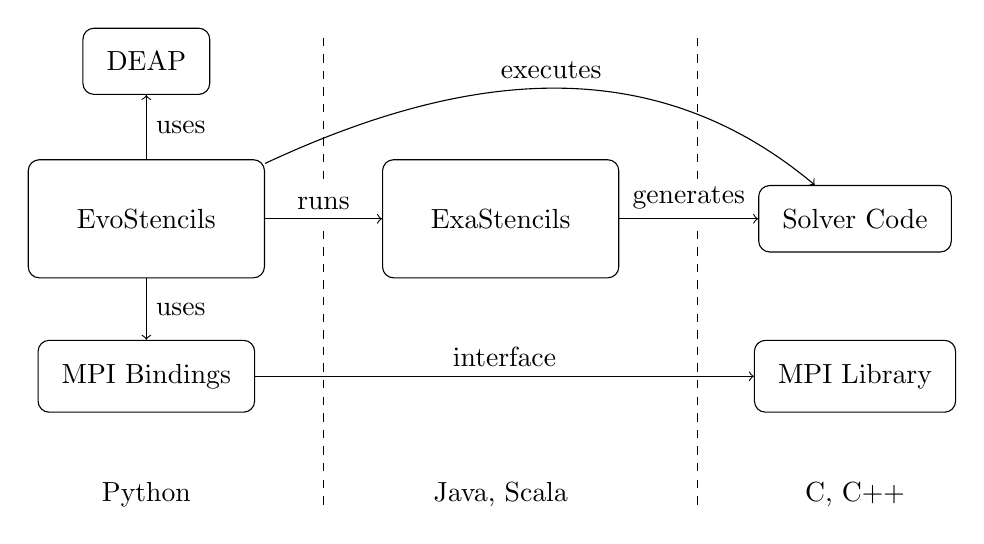
\begin{tikzpicture}
			%\draw [help lines] (-10,-10) grid (10,10);
			\node[draw, minimum width=3cm, minimum height=1.5cm, rounded corners] (evo) at (0,0) {EvoStencils};
			\node[draw, inner sep=3mm, rounded corners] (bindings) at (0, -2) {MPI Bindings};
			\node[draw, inner sep=3mm, rounded corners] (deap) at (0, 2) {DEAP};
			\node[draw, minimum width=3cm, minimum height=1.5cm, rounded corners] (exa) at (4.5, 0) {ExaStencils};
			\node[draw, inner sep=3mm, rounded corners] (code) at (9, 0) {Solver Code};
			\node[draw, inner sep=3mm, rounded corners] (mpi) at (9, -2) {MPI Library};
			\draw[dashed] (2.25, 2.3) -- (2.25,0.5);
			\draw[dashed] (2.25, -0.15) -- (2.25,-3.7);
			\draw[dashed] (7, 2.3) -- (7,0.5);
			\draw[dashed] (7, -0.15) -- (7,-3.7);
			\node (python) at (0, -3.5) {Python};
			\node (java) at (4.5, -3.5) {Java, Scala};
			\node (c) at (9, -3.5) {C, C++};
			\draw[->] (evo)-- node[anchor=west] {uses} (deap);
			\draw[->] (evo)-- node[anchor=south]{runs} (exa);
			\draw[->] (exa)--node[anchor=south] {generates} (code);
			\draw[->] (evo) to [out=25,in=140] node[anchor=south] {executes} (code);
			\draw[->] (bindings)--node[anchor=south] {interface}(mpi);
			\draw[->] (evo)--node[anchor=west] {uses}(bindings);
			%\draw[->] (mpi)--(code);
		\end{tikzpicture}
	}\caption{Software Architecture of EvoStencils.}
	\label{fig:evostencils-architecture}
\end{figure}
In the following, we will now discuss the individual parts of this architecture in more detail, starting with the core implementation of EvoStencils, which can be considered as a separate module that does not depend on any of the other tools and libraries mentioned here.
As a first step, we will outline the implementation of an intermediate representation (IR) for multigrid methods that can be generated in a straightforward manner based on a given derivation tree.
This IR will then act as a basis for all subsequent steps of solver generation and evaluation.

\section{Intermediate Representation}
\label{sec:intermediate-representation}
Before we derive an IR for each component of a multigrid method, note that each of them needs to be defined with respect to the chosen discretization.
%Note that algebraic multigrid methods~\cite{stuben2001introduction,ruge1987algebraic}, which are not considered in this work, represent an exception to this, as they operate on sparse matrix data structures.
In Section~\ref{sec:discretization}, we have already made the assumption of discretizing the underlying PDE on a hierarchy of structured grids.
To identify a grid within this hierarchy, certain information is required, which we store in a \emph{Grid} data structure whose implementation is shown in Listing~\ref{code:ir:grid}.
In general, a structured grid is defined by its \emph{spacing} ($h$) in each dimension and its \emph{size}, i.e., the number of grid points.
In addition, we also include the grid's \emph{level} to identify it within the discretization hierarchy.
Note that in case the grid is uniform, we only need to store a single value for its spacing in each dimension, while otherwise, a value would need to be stored for each pair of grid points.
As the problems considered in this work are all solved on a hierarchy of uniform grids, we focus on this particular case.
\begin{listing}
	\inputminted{python}{evostencils/ir/grid.py}
	\caption{IR: Structured Grid}
	\label{code:ir:grid}
\end{listing}
After defining a data structure that provides all relevant information about a specific grid within the discretization hierarchy, we can start defining expressions that operate on this data structure.
In Listing~\ref{code:ir:abstact-base-class}, a common abstract base class is provided from which all subsequent expression classes are derived.
\begin{listing}
	\inputminted{python}{evostencils/ir/expression.py}
	\caption{IR: Abstract Expression Base Class}
	\label{code:ir:abstact-base-class}
\end{listing}
In addition to the already mentioned \emph{grid} data structure, this class also defines a \emph{shape} for each expression.
From a mathematical point of view, each expression within a multigrid method either computes a matrix or a vector whose shape can be derived recursively from its operands.
This shape is, thus, defined as a pair $(r, c)$, whose first entry $r$ corresponds to the number of rows and the second $c$ to the number of columns of the corresponding matrix.
Note that a vector of size $n$ can simply be considered a matrix of shape $(n,1)$.
Based on this abstract class, we can distinguish between predefined entities, such as the system matrix and right-hand side, and expressions that refer to the mathematical operations defined within a multigrid method.
First of all, Listing~\ref{code:ir:entity} contains the implementation of the \emph{Entity} base class.
\begin{listing}
	\inputminted{python}{evostencils/ir/entity.py}
	\caption{IR: Entity Base Class}
	\label{code:ir:entity}
\end{listing}
In addition to the previously mentioned attributes, this class is also given a \emph{name} to identify the respective entity.
We can then further define classes for representing an approximate solution, right-hand side, and operator, which are shown in the Listings~\ref{code:ir:approximation}~and~\ref{code:ir:operator}.
\begin{listing}
	\inputminted{python}{evostencils/ir/approximation.py}
	\caption{IR: Approximate Solution and Right-Hand Side}
	\label{code:ir:approximation}
\end{listing}
The shape of each of these entities is determined by computing the product of the grid size over all dimensions.
From a mathematical point of view, the \emph{Approximation} and \emph{RightHandSide} classes both represent vectors.
We, thus, only implement the former and make use of inheritance to avoid unnecessary code duplication in the case of the latter.
In addition to the attributes defined in its parent class, an \emph{Approximation} includes a \emph{predecessor} attribute.
However, we postpone the discussion of this attribute's purpose until we implement the actual grammar.
While the two Python classes shown in Listing~\ref{code:ir:approximation} correspond to the solution and right-hand side of a discretized PDE, Listing~\ref{code:ir:operator} represents its operator, given as one or multiple stencil codes.
\begin{listing}
	\inputminted{python}{evostencils/ir/operator.py}
	\caption{IR: Operator}
	\label{code:ir:operator}
\end{listing}
In Section~\ref{subsec:stencil-codes}, we have already introduced a mathematical notation for stencil codes in the form of Equation~\eqref{eq:stencil-definition}, which can be implemented in a straightforward manner leading to the \emph{Stencil} class shown in Listing~\ref{code:ir:stencil}.
%TODO introduce stencil implementation here
\begin{listing}
	\inputminted{python}{evostencils/ir/stencil.py}
	\caption{IR: Stencil}
	\label{code:ir:stencil}
\end{listing}
The \emph{entries} attribute of this class directly corresponds to our definition of a stencil, whereby we use a \emph{tuple} object to represent this mathematical entity in the Python programming language.
Each entry $e_i$ of this object is, thus, given as
\begin{equation}
	e_i = \left(\bm{a}_i, b_i \right),
\end{equation} 
where $\bm{a}_i$ is the offset from the current grid point in each dimension, given as an array of integer values, and $b_i$ the stencil value that corresponds to each offset, stored as a floating point number.
Based on this class, we can then provide an implementation for each stencil operation defined in Section~\ref{subsec:stencil-codes}.
%Furthermore, in accordance with Section~\ref{subsec:systems-of-pdes} and~\ref{subsec:block-smoothing}, we can extend this implementation to systems of PDEs and block smoothers, which will be briefly covered in the next Chapter of this thesis. %TODO insert ref to next chapter here or remove sentence
Now note that in our implementation of the \emph{Operator} class in Listing~\ref{code:ir:operator}, the stencil is not included directly, but instead, we provide a so-called \emph{stencil generator}.
A stencil generator is a function that returns the discretization of an operator on a particular grid in the form of a stencil.
For instance, the finite-difference discretization of the Laplace operator on a two-dimensional uniform grid leads to the stencil 
\begin{equation*}
	\begin{split}
		\Delta_{h,h} = & \; \big\{ \left( \left( 0,0 \right), 4 / h^2 \right), \left(\left(1,0\right), -1/h^2\right), \left(\left(-1,0\right), -1 / h^2\right), \\ & \left(\left(0,1\right), -1/h^2\right), \left(\left(0,-1\right), -1/h^2\right) \big\}_{h,h},
	\end{split}
\end{equation*}
in which the value at each offset depends on the grid spacing $h$.
Furthermore, in certain cases, it is possible to derive the higher-dimensional version of a stencil from its lower-dimensional counterpart, as we have shown in Section~\ref{subsec:restriction-and-prolongation} for the considered prolongation and restriction operators.
Therefore, instead of storing a unique stencil for each individual operator instance, we can parametrize its generation based on the features of the applied discretization by including a reference to the respective generator function.
Finally, as both prolongation and restriction operators transfer information between adjacent grids within a hierarchy of discretizations, they can be considered as a special case of a general operator, which, for instance, leads to a different value of the \emph{shape} attribute.
For this purpose, the class \emph{InterGridOperator}, from which all restriction and prolongation operators are derived, extends the \emph{Operator} class with the required functionality.
For the sake of brevity, the implementation of this class and the respective \emph{Restriction} and \emph{Prolongation} subclasses can be found in Section~\ref{appendix:ir} of the appendix.

After discussing the implementation of the different entities based on which a multigrid method is built, we next shift our attention to the implementation of IR classes for representing the expressions that constitute its computational structure. 
For this purpose, we first provide basic classes for representing unary and binary expressions, which are shown in Listing~\ref{code:ir:unary-expression} and~\ref{code:ir:binary-expression}.
\begin{listing}
	\inputminted{python}{evostencils/ir/unary_expression.py}
	\caption{IR: Unary Expression Base Class}
	\label{code:ir:unary-expression}
\end{listing}
\begin{listing}
	\inputminted{python}{evostencils/ir/binary_expression.py}
	\caption{IR: Binary Expressions Base Class}
	\label{code:ir:binary-expression}
\end{listing}
In both cases, all necessary properties are obtained from the operands of the expression in a recursive manner.
However, since the result of a binary expression depends on the type of operation, we raise an error if this method is not implemented in one of the derived classes. 
To illustrate that the majority of multigrid operations can already be expressed based on these two classes, we have included a number of specific examples in Section~\ref{appendix:ir} of the appendix.
As discussed in Section~\ref{sec:grammar-based-algorithm-generation}, we aim to represent the computational structure of each multigrid method as a redundancy-free directed graph. 
While the previously defined base classes allow us to represent the arithmetic expressions that occur within the correction terms of a multigrid method, there are two operations that require special treatment.
As we have already seen in Figure~\ref{fig:example-three-grid-method-computational-graph}, it is necessary to access previously computed intermediate results on multiple occasions within a multigrid method.
In particular, each time a coarse-grid correction is performed, we have to restore the previous approximate solution and right-hand side on the respective level.
Furthermore, whenever we compute a new residual, the current expression of both the right-hand side and the approximate solution is required.
For this purpose, we implement the classes \emph{Residual} and \emph{Cycle}, which allow us to establish additional references to previously defined expressions within a multigrid method.
Each of these references then corresponds to one of the subgraphs in Figure~\ref{fig:example-three-grid-method-computational-graph} that possess root nodes with multiple incoming edges, i.e., those subgraphs that have been annotated in Figure~\ref{fig:example-three-grid-method-computational-graph-annotated}.
We will later see the complete graph of a multigrid method can be constructed based on these references.
Listing~\ref{code:ir:residual} shows the implementation of the \emph{Residual} class, which contains references to the system operator $A_H$, the current approximate solution $x_H$ and right-hand side $b_H$, where $H$ is the grid spacing on the current level.
Based on these components, we can easily construct the corresponding residual expression $r_H = b_H - A_H x_H$.
\begin{listing}
	\inputminted{python}{evostencils/ir/residual.py}
	\caption{IR: Residual}
	\label{code:ir:residual}
\end{listing}
As a final step in the implementation of our intermediate representation, the \emph{Cycle} class can be found in Listing~\ref{code:ir:cycle}.
\begin{listing}
	\inputminted{python}{evostencils/ir/cycle.py}
	\caption{IR: Multigrid Cycle}
	\label{code:ir:cycle}
\end{listing}
This class represents the execution of a complete multigrid cycle on a particular level.
It, thus, computes a new value for the approximate solution $x_H$ on a particular level with spacing $H$, i.e.,
\begin{equation*}
	x_H = x_H + \omega c_H \; \text{with} \; P,
\end{equation*}
where $c_H$ is a correction term, $\omega$ the relaxation factor and $P$ a partitioning.
Note that $x_H$ and $c_H$ contain all previous computations performed within the given cycle.
To make the right-hand side available in subsequent steps of the method, such as for the computation of the residual, the data structure includes an additional reference to the corresponding object.
Additionally, a reference to the previous state on the next-higher level is needed to restore the expression for the approximate solution and right-hand side after applying a coarse-grid correction.
To better understand the purpose of the \emph{Residual} and \emph{Cycle} class, consider the example shown in Listing~\ref{code:ir:example.py}, which demonstrates the construction of a computational graph based on the IR described in this section.
\begin{listing}
	\inputminted{python}{evostencils/ir/example.py}
	\caption{Example Usage of the Intermediate Representation}
	\label{code:ir:example.py}
\end{listing}
Starting on the original problem on the finest grid, we first store references to the initial approximate solution and right-hand side in a \emph{Cycle} object, which itself is included as a \emph{predecessor} reference in the subsequently created coarse-grid \emph{Cycle} object.
In order to apply the latter as a coarse-grid correction on the finest grid, the original fine-grid \emph{Cycle} object is restored, and its \emph{correction} variable is replaced by the respective expression, which is obtained by applying the prolongation operator to the approximate solution that has been previously computed on the coarse grid.
As this example demonstrates, our IR enables the assembly of the computational graph in a stepwise manner.
However, to automate the process of generating a multigrid method from its grammar-based representation, we must be able to translate any derivation of the grammar into a corresponding IR object.
For this purpose, we utilize the functionality of the evolutionary computation framework DEAP~\cite{rainville2012deap}.
However, before we proceed with this task, we want to address some final remarks about the IR presented in this section.
The main purpose of the implementation presented here is to uniquely represent the computational structure of a multigrid method in the form of a redundancy-free directed graph.
Thus, to be able to construct such a graph in a step-wise manner based on the formal system described in Chapter~\ref{chapter:multigrid-formal-language}, each \emph{Cycle} node needs to include additional references to the current approximate solution and right-hand side.
While this information is important for the construction of the graph, it could later be discarded by replacing each such node with the respective arithmetic expression for computing an updated approximate solution, as it is shown in the \textsc{update} function in Section~\ref{sec:multigrid-state-transitions}.
Preserving these additional references has the advantage of being able to easily traverse the sequence of \emph{Cycle} objects within each graph.
This not only enables us to easily determine the computational structure of a multigrid method by traversing the corresponding graph data structure but also facilitates the identification of potential errors in the implementation.
We, therefore, represent each newly computed approximate solution as a \emph{Cycle} object, which is then referenced in subsequent computational steps of the method.
Also, note that even though the translation of a graph-based representation to an algorithm later requires us to transform each of these objects into an expression for updating the approximate solution, this operation can be performed while traversing the graph and, thus, does not induce a significant overhead within the process of algorithm generation.

\section{Grammar Generation}
According to Section~\ref{sec:multigrid-grammar}, our family of context-free grammars (CFGs) for the generation of multigrid methods consists of three components, a set of terminals, variables, and productions, while additionally, we have to choose a starting symbol $\ps{S}$ from the set of variables.
In Table~\ref{table:grammar-semantics}, we have defined the semantics of each state transition function occurring within the productions listed in Table~\ref{table:multigrid-grammar}.
While each instance of our grammar has to be formulated on a specific grid hierarchy, we have already mentioned that it is possible to define a structurally-equivalent grammar on a different hierarchy of discretizations with the same number of coarsening steps.
By treating the number of coarsening steps as a parameter, we can, thus, automate the process of grammar generation for different problems and discretizations.
For this purpose, we first need to generate the set of terminals that is defined on each level of the hierarchy, which we encapsulate in the class \emph{Terminals} shown in Listing~\ref{code:grammar:terminals}.
\begin{listing}
	\inputminted{python}{evostencils/grammar/terminals.py}
	\caption{Terminals defined on each level.}
	\label{code:grammar:terminals}
\end{listing}
Note that this class comprises a few notable differences compared to our grammar formulation in Section~\ref{sec:multigrid-grammar}.
First of all, since each smoother considered in this work is derived from the system operator, it can be generated automatically within the grammar.
Also, while so far we have abstractly represented the application of the coarse-grid solver in the form of its multiplication with the inverse $A^{-1}_H$ on the coarsest level with spacing $H$, the coarse-grid solver itself can also be considered as a degree of freedom, and, thus, might be provided by the user.
The implementation of a Python class for representing the coarse-grid solver can be found in Listing~\ref{code:ir:coarse-grid-solver}.
\begin{listing}
	\inputminted{python}{evostencils/ir/coarse_grid_solver.py}
	\caption{IR: Coarse-Grid Solver}
	\label{code:ir:coarse-grid-solver}
\end{listing}
Note that each object of this class may additionally contain an expression that represents a complete multigrid method whose finest grid coincides with the coarsest grid of the original method.
This enables the construction of multigrid methods in a hierarchical manner, which means that after obtaining a multigrid method on a certain hierarchy of discretizations, we can employ it as a coarse-grid solver for another multigrid method formulated on top of our original discretization hierarchy.

\subsection{State Transition Functions}
\label{sec:evostencils:state-transition-functions}
As a second step, based on the \emph{Terminals} class, we can implement the state transition functions defined in Section~\ref{sec:multigrid-state-transitions} to construct the IR object of a particular grammar derivation tree.
Listing~\ref{code:grammar:basic-functions} contains the implementation of each of the five state transition functions defined in Table~\ref{table:grammar-semantics}.
\begin{listing}
	\inputminted{python}{evostencils/grammar/base.py}
	\caption{State Transition: Basic Functions}
	\label{code:grammar:basic-functions}
\end{listing}
While each of these implementations is semantically equivalent to the corresponding function definition, certain adaptions are required due to the properties of the \emph{Cycle} class.
In Section~\ref{sec:intermediate-representation}, we have already discussed the advantages of storing the current state of a multigrid method directly within each \emph{Cycle} object.
As a consequence, the application of each state transition function either alters a given \emph{Cycle} object or returns a new object of this type.
The \emph{residual} function, however, represents an exception to this rule since it expects a \emph{state} variable containing an \emph{Approximation} and \emph{RightHandSide} object as its argument.
Note that according to Table~\ref{table:multigrid-grammar}, every derivation ends with computing the residual based on the initial approximate solution $x_h^0$ and right-hand side $b_h$, given in the form of an \emph{Approximation} and \emph{RightHandSide} object, respectively.
In this case, we, therefore, need to pass the initial state 
\begin{equation*}
	Z_h^0 = (x_h^0, b_h, \lambda, \lambda)
\end{equation*} explicitly to the \emph{residual} function.
Since the third and fourth entry of this tuple is empty, in Python, a binary tuple is sufficient to store the respective \emph{Approximation} and \emph{RightHandSide} object.
Even though in all subsequent computations, the first entry of this tuple then consists of a \emph{Cycle} object, for the sake of simplicity, the right-hand side is always included as a second entry.
This decision allows us to employ the same \emph{residual} function within all grammar productions.
As a consequence, also the \emph{update} function needs to be adapted accordingly, such that the respective binary state tuple, in the form of a \emph{Cycle} object for computing a new approximate solution, and the current right-hand side, is returned.
Finally, since the \emph{state} argument of the \emph{coarse\_grid\_correction} function results from an application of the \emph{update} function, it also represents a binary tuple.
We, therefore, need to extract the first entry of this tuple to obtain the corresponding \emph{Cycle} object.
The second main difference is in the implementation of the \emph{update} function compared to its original definition in Table~\ref{table:grammar-semantics} function.
Here we represent the relaxation factor as an index within a uniformly-sampled interval that is included in the respective \emph{Terminal} object.
While we could explicitly store the relaxation factor as a floating point number, its representation accuracy then depends on the underlying floating point format.
Assume we want to encode a certain derivation tree in a string-based format.
This format then later needs to be decoded in a different environment to restore the original information.
If each relaxation factor is stored as a floating point number, we need to ensure that each number is stored with the same accuracy in both environments.
In contrast, an index can always be accurately represented in the form of a single positive integer value.

While Listing~\ref{code:grammar:basic-functions} provides us with the basic functionality to generate an IR representation of arbitrarily-structured multigrid methods, the majority of the productions defined in Table~\ref{table:multigrid-grammar} consists of a combination of two different state transition functions.
For instance, smoothing is performed through the consecutive application of \textsc{apply} and \textsc{update}.
We can simplify the process of grammar generation by identifying each possible combination of state transitions, each of which can then be implemented in a single Python function.
In Definition~\ref{def:elementary-multigrid-operations}, we have already identified the three elementary multigrid operations \emph{smoothing}, \emph{coarsening}, and \emph{coarse-grid correction}.
In Table~\ref{table:multigrid-grammar}, each of these three operations is defined as a combination of two state transition functions.
First, consider Production~\eqref{prod:smoothing}, which is similarly defined on each level and corresponds to the \emph{smoothing} operation in Definition~\ref{def:elementary-multigrid-operations}.
Each of the resulting productions corresponds to the application of an operator
\begin{equation*}
	B_{H} = \left( M_{H} \right)^{-1},
\end{equation*}
where $M_{H}$ is defined based on the splitting $A_{H} = M_{H} + N_{H}$ on a grid with spacing $H$.
While in Table~\ref{table:multigrid-grammar} $M_{H}$ is provided as a terminal symbol, in practice, it can usually be derived from the system operator $A_{H}$.
Therefore, we can implement its generation within the function \emph{generate\_smoother}, which returns a similar splitting for each operator provided as an argument.
The generation of the actual smoothing expression is then performed in the function \emph{smoothing}, which is shown in Listing~\ref{code:grammar:smoothing}.
\begin{listing}
	\inputminted{python}{evostencils/grammar/smoothing.py}
	\caption{State Transition: Smoothing}
	\label{code:grammar:smoothing}
\end{listing}
Similar to Production~\eqref{prod:smoothing}, the implementation of this function consists of a combination of \textsc{apply} and \textsc{update}, whereby we generate $\ps{B_{h}}$ using the function \emph{generate\_smoother}.
To realize different smoothers, we, thus, only need to provide a generator function for each of them.
For instance, Listing~\ref{code:grammar:jacobi} shows how a Jacobi-based smoother can be implemented.
\begin{listing}
	\inputminted{python}{evostencils/grammar/jacobi.py}
	\caption{Example for generating Jacobi-based smoothers}
	\label{code:grammar:jacobi}
\end{listing}
The second basic multigrid operation \emph{coarsening} is realized in a similar way by combining the functions \textsc{apply} and \textsc{coarsening}.
After the former applies a restriction operator to the previously generated residual expression, the latter creates a new \emph{Cycle} object on the next lower level using the restricted residual as a right-hand side.
Next, we need to provide an implementation for Production~\eqref{prod:coarse-grid-correction}, which corresponds to the \emph{coarse-grid correction} operation in Definition~\ref{def:elementary-multigrid-operations}.
Note that in contrast to the state transition function \textsc{cgc}, this operation additionally updates the current approximate solution with the computed correction.
We can realize this behavior by additionally applying the \textsc{update} function, which generates the respective expression based on the given correction term.
Listing~\ref{code:grammar:inter-grid-operations} shows the implementation of Production~\eqref{prod:coarsening} and~\ref{prod:coarse-grid-correction} in the form of the Python functions \emph{restrict\_and\_coarsen} and \emph{update\_with\_coarse\_grid\_correction}.
\begin{listing}
	\inputminted{python}{evostencils/grammar/inter_grid_operations.py}
	\caption{State Transition: Inter-Grid Operations}
	\label{code:grammar:inter-grid-operations}
\end{listing}
In the case of the latter, we have included the prefix \emph{update\_with} to make its implementation distinguishable from the respective state transition function.
Finally, in contrast to the functions implemented so far, which can be applied on multiple levels, on the coarsest level, the only possible operation is the application of the coarse-grid solver, which corresponds to the Productions~\eqref{prod:coarse-grid-solver} and~\eqref{prod:coarse-grid-solver-correction}.
Here, Production~\eqref{prod:coarse-grid-solver} refers to the construction of the coarse problem, similar to the coarsening step defined in Production~\eqref{prod:coarsening}, while Production~\eqref{prod:coarse-grid-solver-correction} performs the actual correction step based on the exact solution obtained on the coarsest grid. 
However, note that only a single production is available for the variable $\ps{c_{16h}}$ in Table~\ref{table:multigrid-grammar}, which means that the two productions are always applied in succession.
We can, therefore, combine the complete process of updating the current approximate solution based on the coarse-grid solver in a single Python function \emph{update\_with\_coarse\_grid\_solver}, whose implementation is shown in Listing~\ref{code:grammar:coarse-grid-solver}.
\begin{listing}
	\inputminted{python}{evostencils/grammar/coarse_grid_solver.py}
	\caption{State Transition: Coarse-Grid Solver}
	\label{code:grammar:coarse-grid-solver}
\end{listing}
For this purpose, similar to the \emph{restrict\_and\_coarsen} function, we first restrict the correction term of a given \texttt{Cycle} object.
The resulting error equation is then solved directly, which is denoted by the application of the coarse-grid solver.
As a final step, the obtained solution is transferred to the next higher level to correct the current approximate solution.
%TODO mention that EvoStencils includes additional functionality not mentioned here
\subsection{Genetic Programming in DEAP}
\label{sec:evostencils-part1:productions}
Finally, to generate the actual grammar, we need to assemble the respective subexpressions for each of the productions contained in Table~\ref{table:multigrid-grammar} based on the terminal and state transition function implementation presented in the last section.
As already mentioned at the beginning of this chapter, we, therefore, make use of the genetic programming (GP) module of the DEAP framework~\cite{rainville2012deap}. 
In principle, DEAP only offers support for untyped and strongly-typed tree-based GP and, therefore, does not allow implementing grammar-guided GP (G3P) directly.
However, as we have already discussed in Section~\ref{sec:gggp-representation}, G3P can be considered as a special variant of strongly-typed GP, whereby each variable that is placed on the left-hand side of a production encodes a unique type.
Before we discuss how the productions in Table~\ref{table:multigrid-grammar} can be mapped to unique types, we need to introduce the relevant constructs already implemented in the framework.
In DEAP, the main data structure to represent a typed GP system is the class \emph{PrimitiveSetTyped}, which defines the rules of how a program can be constructed based on a set of \emph{Primitive} objects.
As each operation must adhere to these rules, it is ensured that only individuals fulfilling the specified type constraints can be generated.
To demonstrate how a grammar can be implemented as a \emph{PrimitiveSetTyped}, we consider the same example grammar used in Section~\ref{sec:gggp-representation}, whose productions are given by
\begin{equation*}
	\begin{split}
		\ps S \; \; \bnfpo & \; \; \ps E \\
		\ps E \; \; \bnfpo & \; \; \text{if} \; \ps B \; \text{then} \; \ps E \; \text{else} \; \ps E \; | \; \ps A \\
		\ps A \; \; \bnfpo & \; \; -\ps A \; | \; (\ps A + \ps A) \; | \; (\ps A - \ps A) \; | \\
		& \; \; (\ps A \cdot \ps A) \; | \; (\ps A / \ps A) \; | \ps{A}^{\ps{A}} \; | \; x \; | \; y \\  
		\ps B \; \; \bnfpo & \; \;  \neg \ps B \; | \; (\ps B \wedge \ps B) \; | \; (\ps B \vee \ps B) \; | \; u \; | \; v.
	\end{split}
\end{equation*}
Listing~\ref{code:grammar:pset-example} shows the corresponding implementation of the function \emph{generate\_grammar}, which generates a \emph{PrimitiveSetTyped} object.
\begin{listing}
	\inputminted[linenos]{python}{evostencils/grammar/pset_example.py}
	\caption{Grammar Generation with DEAP}
	\label{code:grammar:pset-example}
\end{listing}
Here, the first step is to generate a unique type for each symbol that is contained in the set of variables $V = \left\{\ps{E}, \ps{A}, \ps{B} \right\}$, which can be accomplished using Python's builtin \emph{type} function as shown in line~5--7 of Listing~\ref{code:grammar:pset-example}.
Next, in line~8, a new \emph{PrimitiveSetTyped} object is created, in which we set the return type to $\ps{E}$, similar to the choice of the start variable within the grammar.
In line~11--23, we then proceed with defining each production in the form of a \emph{Primitive} objective, which consists of a function, a list of input types, and an output type.
Counterintuitively, the output and not the input type then defines which variable is placed on the left-hand side of each production.
To understand this contradiction, we need to revisit the process of tree initialization in G3P.
As we have seen in Section~\ref{sec:gggp-initialization}, a new derivation tree is generated starting with the variable $\ps{S}$ by recursively selecting productions for each leaf node of the tree that corresponds to a variable.
Similarly, to generate a tree based on a given \emph{PrimitiveSetTyped}, a \emph{Primitive} is picked randomly from those whose output type matches the specified return type.
After extending the tree accordingly, the process is then continued with each of the input types of the chosen \emph{Primitive}.
Therefore, terminating this process at a certain point within the tree requires choosing a \emph{Primitive} with an empty list of input types, which corresponds to a production whose right-hand side does not contain any variables.
In DEAP, such a \emph{Primitive} is called a \emph{Terminal}, which should not be confused with the terminals introduced in Section~\ref{sec:gggp-representation}, which simply refer to each non-variable symbol of a grammar.
To add either a \emph{Primitive} or \emph{Terminal} object to a given \emph{PrimitiveSetTyped}, the \emph{\_add} method can be used.
Additionally, the methods \emph{addPrimitive} and \emph{addTerminal} are also available, which are usually more convenient to use.
In order to make the productions of our example grammar available to the created \emph{PrimitiveSetTyped} object, we, hence, include a \emph{Primitive} for each of them, using the aforementioned function and the previously defined types.
Note that the production
\begin{equation*}
	\ps E \; \; \bnfpo \; \; \ps A
\end{equation*}
is implemented based on the identity function defined in line~12 of Listing~\ref{code:grammar:pset-example}.
After adding a \emph{Primitive} object for each of the grammar's productions, we need to take care of the four symbols $x$, $y$, $u$, and $v$.
We can represent these symbols as objects of the \emph{Terminal} class, which corresponds to a \emph{Primitive} object without any arguments and, thus, an empty list of input types.
Optionally, a \emph{Terminal} object may also refer to a Python symbol, which can be triggered by setting the \emph{symbolic} argument accordingly.
If we assume that each of the four symbols represents an argument to a Python function generated by our grammar, we additionally have to append it to the list of arguments of the corresponding \emph{PrimitiveSetTyped} object.
For this purpose, we define the local function \emph{add\_argument} in line~25--30, which is then utilized in line~32--35 to include each of the four symbols as an argument. 
Note that for each of the two symbols $x$ and $y$, we create two \emph{Terminal} objects that only differ in their return type.
As a consequence, our implementation includes two additional productions
\begin{equation*}
	\ps E \; \; \bnfpo \; \; \ps x \bnfor \ps y,
\end{equation*}
which are not part of the original grammar.
The reason for this adaption is that DEAP's implementation of the \emph{grow} operator, as described in Section~\ref{sec:gggp-initialization}, expects the availability of at least one \emph{Terminal} and \emph{Primitive} object for each type within a \emph{PrimitiveSetTyped}.
In the given case, we only need to include additional \emph{Terminal} objects for the type $\ps{E}$, as the condition is already fulfilled for all other types.
While the example considered here does not require significant adjustments to the structure of the grammar as the type $\ps{E}$ can already be converted to $\ps{E}$ using the identity function, in general, this is not the case.
In particular, according to Table~\ref{table:multigrid-grammar}, for the majority of the variables of our multigrid grammar, only non-terminal productions, i.e., productions that generate strings with at least one variable, are available.
To handle grammars that violate the requirement of having at least one terminal production for each of its variables, we need to adapt DEAP's implementation of the \emph{grow} operator.
The details of this adaptation will be discussed in Section~\ref{sec:evostencils-part1:evolutionary-program-synthesis}, where we will present the implementation of our evolutionary program synthesis method.
Finally, after constructing a \emph{PrimitiveSetTyped} object that corresponds to our example grammar, we can construct a random derivation tree using the \emph{genGrow} function, which corresponds to the aforementioned \emph{grow} initialization operator.
Based on the resulting tree, a function object is then generated using DEAP's \emph{compile} function, which can be executed similarly to any other Python function by providing a value for each of its arguments.
%Similar to \emph{Primitive} objects, a \emph{Terminal} can be added to an existing \emph{PrimitiveSetTyped} using the \emph{addTerminal} method.

\subsection{Variable Encoding}
After introducing the functionality of DEAP's GP module, we can proceed with the actual implementation of the productions of our multigrid grammar, as defined in Table~\ref{table:multigrid-grammar}.
However, before we define a function for constructing the corresponding \emph{PrimitiveSetTyped}, we need to consider the unique structure of our grammar.
As we have discussed in Section~\ref{sec:multigrid-grammar}, Table~\ref{table:multigrid-grammar} is obtained by repeating the same productions on each level for the corresponding set of variables.
In Listing~\ref{code:grammar:terminals}, we have already implemented a data structure that includes all required terminals for a particular level of the discretization hierarchy.
Therefore, instead of initializing a \emph{PrimitiveSetTyped} with the complete set of productions, we can instead add the respective \emph{Primitive} objects on a per-level basis.
Furthermore, note that Table~\ref{table:multigrid-grammar} is defined for a specific number of coarsening steps.
We can, thus, implement a function that iteratively constructs a multigrid grammar independent of the total number of coarsening steps.
This allows us to deploy the same function for the generation of multigrid grammars defined on different discretization hierarchies, for instance, with a different number of coarsening steps.
As in the above example, we first need to generate a unique type for each variable that is defined on a certain level of our grammar.
While in Listing~\ref{code:grammar:pset-example}, we have encoded each variable with an actual Python type, at this point, we have to introduce an additional constraint that prevents us from pursuing the same approach.
In order to store the state of a program in the form of a serialized binary format, Python provides the \emph{pickle} module.
This module enables the serialization of arbitrary Python objects, which can then later be restored.
Object serialization has multiple purposes in our implementation.
First of all, we want to be able to store the current state of our evolutionary algorithm such that, for instance, in case of a hardware failure, we can continue at the same position.
Furthermore, parallelizing certain parts of our implementation on a distributed computing system using the Message Passing Library (MPI) requires us to transfer arbitrary Python objects via a communication network.
The pickle module provides a simple and portable solution to this problem.
Unfortunately, pickle enforces a number of additional constraints on the serializability of a Python object.
In particular, Python types can only be serialized if they are defined at the top-level domain of a module.
Since our goal is to create a \emph{PrimitiveSetTyped} object adapted to the properties of a grammar that is only provided during program execution, we need to create the respective types dynamically.
Unfortunately, dynamic types can not be defined at the top-level domain of the corresponding Python module, which renders their serialization impossible.
To resolve this issue, we propose a custom \emph{Type} class which is defined in Listing~\ref{code:grammar:typing}.
\begin{listing}
	\inputminted{python}{evostencils/grammar/typing.py}
	\caption{Type Wrapper}
	\label{code:grammar:typing}
\end{listing}
Since the instances of this class are regular Python objects, a pickle-based serialization can be achieved without any further adaption.
To distinguish different \emph{Type} objects within a \emph{PrimitiveSetTyped}, the \emph{identifier} attribute is provided.
In addition, the class also includes a \emph{guard} attribute in the form of a boolean variable, whose purpose will be discussed later in this section. 
To enable type equivalence checking in an automatic manner, we provide a custom \emph{\_\_eq\_\_} method.
We first check whether the other object is also an instance of the \emph{Type} class, as we want to be able the compare a given \emph{Type} object to any other Python object.
If this condition is fulfilled, we then proceed to check if both the \emph{identifier} and \emph{guard} attributes of the \emph{Type} objects are equal.
In order to correctly store \emph{Type} objects in a Python dictionary, we implement the \emph{\_\_hash\_\_} method, where we utilize Python's builtin \emph{hash} function to generate a unique value based on the content of the two attributes. 
Finally, to ensure that the type checking is performed correctly, we adapt the original implementation of the \emph{PrimitiveSetTyped} class such that types are compared using the equality operator instead of Python's built-in \emph{issubclass} function.
The resulting implementation can be found in Section~\ref{appendix:gp} of the appendix.

Based on this tailored type representation, we can now implement a data structure that incorporates the type of each variable defined on a given level.
The implementation of this data structure in the form of the \emph{Types} class is shown in Listing~\ref{code:grammar:types}.
\begin{listing}
  	\inputminted[linenos]{python}{evostencils/grammar/types.py}
  	\caption{Data Structure for Variable Types}
  	\label{code:grammar:types}
\end{listing}
%TODO include line numbers at the respective text positions
To initialize the type that corresponds to a certain variable of the grammar, we can either create a new \emph{Type} object based on an \emph{identifier} or retrieve the respective object if it is already contained in the \emph{Types} object that refers to the next higher level in the discretization hierarchy.
The resulting initialization procedure is implemented in the \emph{\_init\_type} method, which can be found in line~2--9 of Listing~\ref{code:grammar:types}.
By applying this function, we obtain a \emph{Type} object with unique \emph{identifier} for each variable defined on two subsequent levels of the discretization hierarchy, whereby each attribute with a subscript $h$ and $2h$ corresponds to a variable on the current and next coarser level, respectively.
Consequently, if we provide an existing \emph{Types} object for the initialization of its predecessor on the next lower level, the coarse-grid types correspond to the fine-grid types of this object.
We, therefore, only have to generate a unique type for each variable once, which can then be transferred to a lower level in the form of a reference to the respective \emph{Type} object.
For the sake of simplicity, we identify each \emph{Type} object with a Python \emph{string}. 
The resulting generation of each \emph{Type} object and its assignment to the respective attribute is performed in line~13--33.
In contrast to the types that need to be defined on each level, both the \emph{Partitioning} and \emph{RelaxationFactorIndex} attribute is level-independent, and, thus, only a single type needs to be created for each of them, which is shown in line~36 and~37.

\subsection{Productions}
With the implementation of a type system that allows expressing each production as a mapping between input and output types, we are now finally at the point where we can bring everything together.
Similar to the example shown in Listing~\ref{code:grammar:pset-example}, we first have to create a \emph{PrimitiveSetTyped} to which we can then add the respective \emph{Terminal} and \emph{Primitive} objects in an iterative manner.
The resulting implementation is shown in Listing~\ref{code:grammar:init-grammar}.
\begin{listing}
	\inputminted[linenos]{python}{evostencils/grammar/init_grammar.py}
	\caption{Grammar Initialization}
	\label{code:grammar:init-grammar}
\end{listing}
In line~6--14, we first construct the respective \emph{Terminals} and \emph{Types} data structures on the finest grid of the given discretization hierarchy.
Based on these data structures, we proceed with the creation of the \emph{PrimitiveSetTyped} object in line~15.
In line~16--21, we then include the initial state as a tuple consisting of the respective \emph{Approximation} and \emph{RightHandSide} object and a number of level-independent terminals.
For the sake of simplicity, we assume that it is possible to generate all required \emph{Approximation}, \emph{RightHandSide} and \emph{Operator} objects using a predefined \emph{Generator} class, which retrieves the required information automatically from a domain-specific representation of the problem.
All other \emph{Terminal} and \emph{Primitive} objects are then included in line~23 using the \emph{add\_level} function shown in Listing~\ref{code:grammar:add-level}.

At this point, we now need to come back to the definition of the \emph{Type} class, which includes an additional \emph{guard} attribute.
The purpose of this attribute is to enforce additional constraints that are not present in the productions in Table~\ref{table:multigrid-grammar}.
Consider, for instance, the derivation
\begin{equation*}
\ps{S} \Rightarrow \ps{s_h} \Rightarrow (x_h^0, b_h, \bnfes, \bnfes),
\end{equation*}
which is valid according Table~\ref{table:multigrid-grammar}.
However, the resulting method consists only of a single statement, which returns the initial approximate solutions.
It is, thus, important to define the minimal requirements a sequence of operations needs to fulfill to qualify as a multigrid method. 
While the optimal amount of smoothing and coarse-grid corrections might differ for each case, we consider it essential to apply the coarse-grid solver at least once to obtain an accurate approximation of the solution of the error equation on the coarsest grid.
We can enforce this requirement with the mentioned \emph{guard} attribute of the \emph{Type} class.
As each derivation of our grammar ends with the generation of the initial state $\left(u_h^0, b_h\right)$ on the finest level, we have to prevent the application of the respective production until the coarse-grid solver has been utilized at least once.
For this purpose, we set the output type of the respective \emph{Terminal} object in line~16 of Listing~\ref{code:grammar:init-grammar} to the \emph{S\_guard\_h} attribute of the respective \emph{Types} data structure.
We then define all remaining productions in such a way that all possible derivations include the function \emph{update\_with\_coarse\_grid\_solver}, as shown in Listing~\ref{code:grammar:coarse-grid-solver}, at least once.
Listing~\ref{code:grammar:add-level} demonstrates how this can be achieved for each level within a discretization hierarchy of arbitrary depth.
\begin{listing}
	\inputminted[linenos]{python}{evostencils/grammar/add_level.py}
	\caption{Terminal and Primitive Generation per Level}
	\label{code:grammar:add-level}
\end{listing}
In line~2, we first make use of the function \emph{add\_terminals}, whose implementation is shown in Listing~\ref{code:grammar:add-terminals}, to add all terminals that are required on the respective level to the given \emph{PrimitiveSetTyped}.
\begin{listing}
	\inputminted{python}{evostencils/grammar/add_terminals.py}
	\caption{Terminal Generation per Level}
	\label{code:grammar:add-terminals}
\end{listing}
To facilitate the process of generating  \emph{Primitive} objects, we implement the helper function \emph{add\_primitive} in line~4--6.
This function can generate multiple instances of the same \emph{Primitive} using different input and output types, which we utilize to include each type as a guarded and unguarded version.
Now note that each derivation starts with \emph{S\_h} and ends with the type \emph{S\_guard\_h}.
According to the productions in Table~\ref{table:multigrid-grammar}, only four unique primitives are required on each level, except for the definition of different smoothers.
For each of the \emph{Primitive} objects generated lines~9--17 whose list of input types contains only unguarded types, the output type is also unguarded.
Consequently, so far, with none of the generated \emph{Primitive} objects, a transition from an unguarded to a guarded type is possible.
We can, thus, enforce that the coarse-grid solver is applied at least once within each derivation by including the necessary transition in line~20.
Since this transition represents the only way to reach the final state, the application of the \emph{update\_with\_coarse\_grid\_solver} function is a necessary requirement for the termination of each derivation.
Note that we only want to add this production on the lowest level, where it replaces the respective productions for the coarsening and coarse-grid correction steps.
We, therefore, have to check whether we have reached the lowest level of the discretization hierarchy, which is done in line~15 of Listing~\ref{code:grammar:add-level}.
Since we generate the respective \emph{Primitive} additionally with an unguarded input type, similar to most other productions, the coarse-grid solver can be applied multiple times within each derivation.

Finally, using the functions \emph{init\_grammar} and \emph{add\_level}, we can define the Python function \emph{generate\_grammar}, whose implementation is shown in Listing~\ref{code:grammar:generate-grammar}. 
This function generates a \emph{PrimitiveSetTyped} for discretization hierarchies of variable depth.
\begin{listing}
	\inputminted[linenos]{python}{evostencils/grammar/generate_grammar.py}
	\caption{Grammar Generation}
	\label{code:grammar:generate-grammar}
\end{listing}
%TODO maybe clarify the meaning of max_level in comparison to earlier sections
In line~8--10, we first construct an initial \emph{PrimitiveSetTyped} to which we add all required \emph{Terminal} and \emph{Primitive} objects on the finest grid using the previously defined function \emph{init\_grammar}.
In case the given discretization hierarchy consists of at least three levels, we iteratively extend our \emph{PrimitiveSetTyped} using the \emph{add\_level} function.
For this purpose, we only have to create the respective \emph{Terminals} and \emph{Types} data structures, as shown in lines~10--20, which are then passed to \emph{add\_level} in order to generate all required \emph{Primitive} and \emph{Terminal} objects.
After we have traversed all levels, the \emph{PrimitiveSetTyped} object returned at the end of the function precisely replicates the functionality of Table~\ref{table:multigrid-grammar} formulated on the given hierarchy of discretizations.

\section{Evolutionary Program Synthesis}
\label{sec:evostencils-part1:evolutionary-program-synthesis}
In order to provide an accessible interface to EvoStencils' functionality, we implement all steps from the construction of a grammar, based on the given PDE-based problem, to the synthesis of an optimal program in the \emph{Optimizer} class, whose basic implementation is shown in Listing~\ref{code:optimization:optimizer}.
\begin{listing}
	\inputminted[linenos]{python}{evostencils/optimization/optimizer.py}
	\caption{Optimizer class}
	\label{code:optimization:optimizer}
\end{listing}
In addition to the generated \emph{PrimitiveSetTyped} object, this class relies on two main components, a \emph{Toolbox} object for the execution of the evolutionary program synthesis and a \emph{ProgramGenerator} object, which enables the generation and evaluation of solver implementations while also providing an interface to all required information about the given PDE-based problem, for instance, in the form of the respective operators.
Based on the functionality of these two components, which, in the following, will be described in detail, we can implement a \emph{run} method, which first generates a \emph{PrimitiveSetTyped} and then, based on the initialized \emph{Toolbox} object, performs an evolutionary program synthesis that yields a population of individuals representing efficient multigrid methods for the given problem.
Note that within this procedure, the evaluation of each generated solver relies on an \emph{evaluate} method, which returns suitable metrics for assessing its quality.

After translating our class of multigrid grammars introduced in Section~\ref{sec:multigrid-grammar} into a strongly-typed GP system, we can now make use of the functionality of DEAP's GP module to implement the evolutionary search operators introduced in Section~\ref{sec:gggp}.
However, before we can define each operator, we first need to implement a data structure for storing a derivation tree generated based on the rules of our grammar.
For this purpose, DEAP provides the \emph{PrimitiveTree} class, which represents each tree as a list of \emph{Primitive} and \emph{Terminal} objects stored in depth-first order.
Each entry of this list, thus, corresponds to the choice of a particular production in the form of a \emph{Primitive} or \emph{Terminal} object, while its return type refers to the respective variable on the left-hand side.
Therefore, each node of the tree this list represents refers to a certain variable and its children within the derivation tree.
After obtaining a suitable data structure for the representation of each derivation tree generated by our grammar, the next step is the randomized creation of an initial population.
As we have already discussed in Section~\ref{sec:gggp-initialization}, the \emph{full} initialization operator~\cite{koza1994genetic,poli2008field} is only applicable in cases where a grammar enables the termination of unfinished branches at any given point in the derivation by invoking a terminal production.
However, as it can be seen in Table~\ref{table:multigrid-grammar}, not all variables of our grammar fulfill this condition.
For instance, the variable $\ps{c_h}$ always yields a residual expression containing $\ps{s_h}$.
In contrast, the \emph{grow} operator is a suitable initialization operator in the given case, as it supports the generation of trees with branches of variable length. 
The DEAP framework implements random tree generation in the \emph{generate} function, which constructs a tree based on a given \emph{PrimitiveSetTyped} object while enforcing that the length of each of its branches satisfies a certain depth limit.
If a certain branch satisfies this limit, this function always tries to pick a \emph{Terminal} object among the available productions to finish the growth at the respective branch. 
Note that these productions are given in the form of a list of \emph{Primitive} and \emph{Terminal} objects whose output types match with the input type of the node from which the current branch should be grown further.
Unfortunately, the specified limit is applied in a strict sense, and thus, the \emph{generate} function fails if a \emph{Terminal} object is erroneously expected to be available for a certain type.
To resolve this issue, we, therefore, need to adapt DEAP's implementation of the \emph{generate} function, such that the specified limit is only applied whenever possible.
In order to circumvent cases where the constraint of choosing only \emph{Terminal} objects can not be satisfied, we simply ignore it for the current step, which means that we extend the given node with a random \emph{Primitive}.
We then proceed with the current branch while choosing a \emph{Terminal} object whenever possible until the growth finally ends.
As an additional option, we also allow the insertion of an existing branch into the generated tree, which corresponds to the \emph{subtree insertion} operator already discussed in Section~\ref{sec:gggp-mutation-and-recombination}.
Based on the \emph{generate} function, we can then finally implement the \emph{grow} operator in the form of the function \emph{genGrow}, which chooses the maximum depth of a tree randomly from an interval defined by the parameters \emph{min\_height} and \emph{max\_height}.
The resulting implementation is shown in Listing~\ref{code:gp:grow}, while the \emph{generate} function can be found in Section~\ref{appendix:gp} of the appendix.
\begin{listing}[!htb]
	\inputminted{python}{evostencils/gp/grow.py}
	\caption{GP: Grow operator}
	\label{code:gp:grow}
\end{listing}
In order to prevent the random generation of excessively large expressions, the \emph{genGrow} function additionally enforces a size limit, which, by default, is set to 150.
Therefore, if a generated tree does not fulfill this constraint, we repeat the process, again starting from scratch, until the requirement is met for one of the resulting trees.

\subsection{Evolutionary Operators}
Based on our implementation of the \emph{generate} function and DEAP's built-in functionality, we can now define all remaining components of an evolutionary program synthesis method.
To facilitate the utilization of different operator choices within the context of an evolutionary search method, DEAP provides the \emph{Toolbox} container for the creation of unified interfaces.
Listing~\ref{code:gp:toolbox} demonstrates how we generate such a container for the given case.
\begin{listing}
	\inputminted[linenos]{python}{evostencils/gp/toolbox.py}
	\caption{GP: Toolbox initialization}
	\label{code:gp:toolbox}
\end{listing}
First of all, we define a data structure for the fitness of each individual based on DEAP's built-in \emph{Fitness} class.
Here, the \emph{weights} attribute determines the number of objectives, while a negative value means that the respective objective is to be minimized.
As we will later come back to the definition of the optimization objectives, at this point, the reader can just assume that either a single or a multi-objective minimization is performed.
Next, as we have already discussed previously, we represent each \emph{Individual} as a \emph{PrimitiveTree}, whereby we set the \emph{fitness} attribute to the previously defined data structure.
To facilitate the implementation of both the \emph{Fitness} and \emph{Individual} class, in lines~6--10, we make use of DEAP's \emph{creator} module.
For a detailed description of the functionality of this module, the reader is referred to the documentation of the DEAP framework\footnote{DEAP Creator Module: \url{https://deap.readthedocs.io/en/master/api/creator.html}}.
Based on the definition of these two classes, we can then create the actual \emph{Toolbox} object together with all evolutionary operators.
To generate a random individual, we apply our custom \emph{genGrow} function, as described above.
A complete population can then be generated by utilizing DEAP's \emph{initIterate} and \emph{initRepeat} functions~\footnote{DEAP Evolutionary Tools: \url{https://deap.readthedocs.io/en/master/api/tools.html}}.
Next, we implement suitable crossover and mutation operators for our tree-based G3P method, as defined in Section~\ref{sec:gggp-mutation-and-recombination}.
For the former, we apply subtree crossover for which an implementation is already available in the form of the function \emph{cxOnePoint} of DEAP's GP module.
To implement subtree replacement and insertion within a single function, we, again, utilize our custom \emph{generate} function, which already provides the required functionality.
The resulting implementation of the function \emph{mutateSubtree} is shown in Listing~\ref{code:gp:mutate}.
\begin{listing}[!htb]
	\inputminted{python}{evostencils/gp/mutate.py}
	\caption{GP: Subtree mutation operator}
	\label{code:gp:mutate}
\end{listing}
Similar to the \emph{genGrow} function, \emph{mutateSubtree} includes an interval from which the maximum depth of the newly generated subtree is chosen.
To prevent the size of the inserted subtree from exceeding the size of the original tree, usually, a smaller interval is chosen than for the \emph{genGrow} function, for instance, with only half the size.
Now before we can implement the actual evolutionary search method, we need to address the problem of selecting promising individuals for recombination and mutation.
Therefore, we first need to find a way to accurately evaluate the quality of a multigrid method in an automatic manner.

\subsection{Fitness Evaluation and Selection}
\label{sec:fitness-evaluation-and-selection}
In Section~\ref{sec:grammar-based-algorithm-generation},
we have already demonstrated that it is possible to obtain the algorithmic representations of a multigrid method based on a computational graph similar to the one shown in Figure~\ref{fig:example-three-grid-method-computational-graph}.
In Section~\ref{sec:intermediate-representation}, we have then introduced an intermediate representation (IR) for multigrid methods that stores each computational graph as a hierarchical composition of \emph{Cycle} objects, as demonstrated by the example shown in Listing~\ref{code:ir:example.py}.
Consequently, similar to the discussion in Section~\ref{sec:grammar-based-algorithm-generation}, we can translate each multigrid method, given as a \emph{Cycle} object generated by the respective grammar, to an algorithmic representation.
This translation is performed by traversing the given hierarchy of IR objects in a recursive bottom-up manner.
However, we still need to address the question of how we can evaluate a multigrid method based on this representation, which requires us to define one or multiple metrics for assessing its quality.
For this purpose, we first have to revisit the general notion of an iterative method, as defined in Section~\ref{sec:basic-iterative-methods}.
In principle, an iterative method for solving the linear system $A \bm{x} = \bm{b}$ is characterized by the repeated application of a number of well-defined computational steps, whereby each step has the purpose of computing an improved approximation $\tilde{\bm{x}}$ for the solution of the system based on the previous one.
If we execute an iterative solver on a given computing system, usually the goal is to approximate the solution of the target problem up to a certain accuracy in as little time as possible, which we define as the \emph{solving time} $T_{\varepsilon}$, where $\varepsilon$ is the desired reduction of the initial error. 
Furthermore, if we assume that an iterative method performs the same sequence of computations in each of its iterations, we can define the solving time as
\begin{equation}
	T_{\varepsilon} = t \cdot n_{\varepsilon},
	\label{eq:solving-time-basic}
\end{equation} 
where $t$ is the execution time of each iteration of the method and $n_{\varepsilon}$ the number of iterations required to achieve an error reduction of $\varepsilon$.
Note that in contrast to $n_{\varepsilon}$, the execution time $t$ solely depends on the amount of computations performed within each iteration and is, hence, independent of $\varepsilon$.
Next, similar to Section~\ref{sec:basic-iterative-methods}, we define the \emph{convergence factor} of an iterative method as the limit of the sequence
\begin{equation*}
	\rho = \lim \limits_{n \to  \infty} \Bigg( \underbrace{ \max \limits_{x^{(0)} \in \mathbb{R}^{n}} \frac{\norm{\bm{x}^{(n)} - \bm{x}^{*}}}{\norm{\bm{x}^{(0)} - \bm{x}^{*}}} }_{\varepsilon_n} \Bigg)^{\frac{1}{n}},
\end{equation*}
where $\varepsilon_n$  is the minimum error reduction after $n$ iterations of the method.
Similarly, we can define the iteration-dependent convergence factor
\begin{equation}
	\rho_n = \left( \varepsilon_n \right)^{\frac{1}{n}}.
	\label{eq:iteration-dependent-convergence-factor}
\end{equation} 
Now assume that our goal is to achieve an error reduction $\varepsilon$.
Therefore, we can set $\varepsilon_n = \varepsilon$ and apply the natural logarithm to both sides of Equation~\eqref{eq:iteration-dependent-convergence-factor} which yields
\begin{equation*}
	n = \frac{\ln \varepsilon}{\ln \rho_n},
\end{equation*} 
where $n$ now represents the required number of iterations to achieve an error reduction of $\varepsilon$.
Since, for a given convergence factor $\rho_n$, the number of iterations $n$ can now be considered as a function of $\varepsilon$, we can insert the resulting term into Equation~\eqref{eq:solving-time-basic} and obtain
\begin{equation*}
	T_{\varepsilon} = t \cdot n_{\varepsilon} = t \cdot \frac{\ln \varepsilon}{\ln \rho_{n_{\varepsilon}}}.
\end{equation*} 
If we additionally assume that $\rho_{n_{\varepsilon}} \approx \rho$ for a sufficiently high number of iterations, we can further simplify this equation to
\begin{equation}
	T_{\varepsilon} = t \cdot n_{\varepsilon} = t \cdot \frac{\ln \varepsilon}{\ln \rho}.
	\label{eq:solving-time}
\end{equation} 
Now note that since the negative value of the natural logarithm decreases between zero and one, a smaller convergence factor leads to a faster solving time.
For example assume achieving an error reduction of $\varepsilon = 10^{-6}$ using an iterative method with a convergence factor of $\rho = 0.5$ would require 20 iterations, while with a convergence factor of $\rho = 0.1$ the same accuracy could be achieved in only six iterations.
Consequently, there are, in principle, two possibilities to improve upon an existing solver by reducing its execution time $t$ or convergence factor $\rho$. 
However, as we have discussed in Section~\ref{sec:multigrid-cycles}, the choice of each method usually represents a compromise between a lower number of computations and, thus, a faster execution time and a faster convergence, which usually requires more computations.

While we have now discussed how to assess the quality of an iterative method, we have not yet answered how to choose one or multiple optimization objectives based on these metrics.
In addition to achieving a fast solving time, the main goal of automated algorithm design is \emph{generalization}, which means that we aim to find multigrid methods that are robust in solving problems with similar characteristics.
Theoretically, we could simply execute a solver on each individual problem instance of interest and then measure its solving time.
However, due to the high computational demands of solving PDEs in many domains, this approach is often infeasible.
One way to mitigate this issue is the application of \emph{predictive models} to obtain an estimation without the need to actual execute the solver on any problem.
While the latter approach is usually faster to execute, its application to non-standard multigrid cycles, as the one shown in Figure~\ref{fig:non-traditional-multigrid-cycle}, is not well-researched.
Due to the entirely different nature of the two performance-guiding metrics $t$ and $\rho$, we need to consider them separately.
First of all, note that the execution time $t$ of each step of an iterative method depends entirely on the amount of computations and their execution efficiency on the given compute platform.
In contrast, the convergence factor $\rho$ is linked to the mathematical properties of the solver, for instance, its capability to quickly reduce certain error components, as we have discussed in Section~\ref{sec:multigrid-methods}. 
While the availability of performance models for modern computer architectures, as the roofline~\cite{williams2009roofline} and execution-cache memory model~\cite{hager2016exploring}, enables predictions in an automated and deterministic manner, analyzing the mathematical properties of a solver is often difficult.
Local Fourier analysis (LFA)~\cite{wienands2004practical} represents a promising approach for predicting the convergence behavior of an iterative solver in a resolution-independent manner.
Even though LFA has already been applied successfully to numerous applications~\cite{rodrigo2017validity}, only recently software tools that automate its execution have become available~\cite{rittich2018extending,kahl2020automated}.
In~\cite{schmitt2020constructing,hoefer2020comparing}, we have performed a number of experiments to test whether the library LFA Lab~\footnote{LFA Lab: \url{https://github.com/hrittich/lfa-lab}} is suitable for the automated convergence estimation of grammar-generated multigrid methods.
While LFA Lab yields reliable predictions for many model problems and common multigrid cycles, unfortunately, we could not obtain the same degree of accuracy for many non-standard cycles and more complicated problems, such as systems of PDEs.

A second option to decrease the cost of the evaluation is to estimate the quality of a given solver by measuring its characteristics on a number of proxy problems that are faster to solve than the original problem while possessing similar mathematical properties.
One of the main features of multigrid is that, if properly constructed, these methods can achieve $h$-independent convergence, which means that we can apply the same solver to a larger instance of the same problem without slowing down its convergence~\cite{trottenberg2000multigrid}.
Therefore, in case our goal is to solve a certain PDE discretized on a grid with step size $h$, we can instead consider an instance of the same PDE on a similar grid with lower resolution and, thus, a larger spacing of the grid points.
If a given multigrid method is able to achieve $h$-independent convergence on a sequence of increasingly finer resolved instances of the same PDE, there is a high probability that the method also generalizes to other problem instances.
However, the application of this approach requires us to generate efficient implementations for each multigrid method considered, which can then be executed to obtain the relevant quality metrics on each proxy problem.
For this purpose, we must be able to automate the process of generating a solver implementation based on its algorithmic representation.
Recently, code generation techniques that grant us this capability have become available~\cite{kostler2020code,schmitt2018automating}.
ExaStencils\footnote{ExaStencils: \url{https://www.exastencils.fau.de}} is a code generation framework, implemented in the Scala programming language, that has been specifically designed for the automatic generation of scalable multigrid solver implementations on modern parallel computing hardware~\cite{lengauer2014exastencils,lengauer2020exastencils}.
It enables the formulation of multigrid methods in a discretization-independent domain-specific language (DSL) called ExaSlang~\cite{schmitt2014exaslang,schmitt2016systems}, which is almost indistinguishable from the textbook-like description of an algorithm.
Based on this DSL specification, the framework is able to generate highly-optimized C++ code for different problem sizes and computer architectures.
To illustrate this approach, Listing~\ref{code:exaslang-example} shows an ExaSlang implementation of the three-grid method formulated in Algorithm~\ref{alg:example-three-grid-method}.
\begin{listing}
	\inputminted[fontsize=\footnotesize,breaklines]{scala}{evostencils/code_generation/three_grid_example.exa3}
	\caption{Three grid example from Algorithm~\ref{alg:example-three-grid-method} in ExaSlang}
	\label{code:exaslang-example}
\end{listing}
As this example demonstrates, ExaSlang enables the formulation of the same operations on different levels of a discretization hierarchy based on so-called \emph{level declarations}\footnote{In case no level declaration is provided, ExaStencils assumes that the operation is applied on the current level.}.
Similar to the specification of the grid spacing as a subscript in Algorithm~\ref{alg:example-three-grid-method}, we can utilize this notation to formulate each operation within a multigrid method relative to the \emph{finest} grid.
Since the ExaSlang specification of a multigrid method is, thus, independent of the actual discretization width, the ExaStencils compiler is able to generate implementations of the same solver for different grid sizes.
Furthermore, as ExaSlang supports the formulation of each multigrid operation in a high-level mathematics-like syntax, we can also apply the same solver to different problems only by changing the definitions of the individual operators, such as the system, prolongation, and restriction operator.
Therefore, ExaStencils is ideally suited for the automatic generation and evaluations of multigrid methods within our evolutionary program synthesis approach.
While ExaStencils is implemented in the Scala programming language and can, thus, not be accessed directly within Python code, it provides simple configuration files, which allow us to adapt certain problem characteristics, such as the grid spacing and the number of coarsening steps.
Furthermore, additional code generation options, such as compiler-based performance optimizations, can be en- or disabled.
To encapsulate the usage of the ExaStencils compiler, EvoStencils provides the \emph{ProgramGenerator} class.
In addition to the automatic adaption of the respective configuration files and the actual execution of the code generation process, this class also includes functionality for extracting the required information about a given problem based on an existing ExaSlang specification. 
Therefore, if this specification contains all the necessary information for the generation of the respective multigrid grammar, it allows us to integrate EvoStencils directly into ExaStencils' solver generation workflow.
This approach, furthermore, enables the application of our evolutionary program synthesis method to many of the problems that are already available within ExaStencils.
Based on the functionality provided by the \emph{ProgramGenerator} class, we can implement an evaluation function in the form of the \emph{evaluate} method of the previously mentioned \emph{Optimizer} class.
The implementation of this method is shown in Listing~\ref{code:optimization:evaluate}.
\begin{listing}
	\inputminted[fontsize=\footnotesize,breaklines]{scala}{evostencils/optimization/evaluate.py}
	\caption{}
	\label{code:optimization:evaluate}
\end{listing}
It provides a high-level interface to the evaluation of an arbitrary individual generated based on the provided \emph{PrimitiveSetTyped} object.
First of all, in order to prevent the repeated evaluation of structurally-equal individuals, the \emph{Optimizer} class implements a caching mechanism that keeps track of all previously evaluated individuals.
Therefore, we first check whether the given individual has already been evaluated before, in which case we simply return the cached objective function value.
Otherwise, we utilize the \emph{generate\_and\_evaluate} method of the \emph{ProgramGenerator} class to generate a C++ implementation of the corresponding solver using the ExaStencils compiler, which is then executed on a proxy problem.
As a result, we obtain three metrics, the total solving time $T_\varepsilon$, the convergence factor $\rho$, and the number of iterations $n_\varepsilon$, whereby the desired error reduction $\varepsilon$ is usually determined by the given ExaStencils specification of the problem.
As, in general, the solution of the given PDE is not known in advance, we approximate the convergence factor using the formula
\begin{equation}\label{eq:asymptotic_convergence_factor}
	\rho \approx \left(\prod_{i=1}^{n}\tilde{\rho}_i \right)^{1/n},
\end{equation} where $n$ is the number of iterations until convergence and
\begin{equation*}
	\tilde{\rho}_{i} = \frac{\norm{b_h - A_h x_{h}^i }}{\norm{b_h - A_h x^{i-1}_{h}}}
\end{equation*}
is the L2-norm of the residual reduction in every iteration of the solver~\cite{trottenberg2000multigrid}.
To determine the execution time per iteration $t$ of the method, we simply divide the total solving time by the number of iterations.
To reduce potential hardware-based variations in the execution of each solver, $T_\varepsilon$ is obtained as an average over multiple evaluations of the same individual.
Note that, at this point, we assume that a multi-objective optimization is performed, as the returned \emph{Fitness} object includes two objectives.
However, it is also possible to implement a similar function that returns a single-objective fitness value, for instance, in the form of the total solving time.
Finally, the method enables the adaption of certain parameters of the underlying PDE for the current evaluation.
For this purpose, a mapping from each parameter to the respective value can be provided in the form of a Python dictionary.

After successfully obtaining a \emph{Fitness} object for each individual, we can complete our collection of evolutionary operators with the definition of suitable selection and elitism methods.
As we have discussed in Section~\ref{sec:gggp-evaluation-and-selection}, in contrast to initialization, mutation, and crossover, the selection of individuals within an evolutionary algorithm is independent of their underlying representation, but solely depends on the definition of their fitness.
Therefore, different selection operators have been proposed for single and multi-objective evolutionary algorithms, of which many are already available within the DEAP framework.  
Similar to the other evolutionary operators in Listing~\ref{code:gp:toolbox}, we can add a certain selection operator to a given \emph{Toolbox} object, by using its \emph{register} method.
Listing~\ref{code:optimization:selection} shows the example initialization of a \emph{Toolbox} object using the widely-used NSGA-II selection operator~\cite{deb2002fast}. 
\begin{listing}
	\inputminted[linenos]{python}{evostencils/optimization/selection.py}
	\caption{Example for Multi-Objective Selection}
	\label{code:optimization:selection}
\end{listing}
In a similar manner, we can initialize a \emph{Toolbox} object with arbitrary different single- and multi-objective selection operators and evaluation functions based on the definition of the \emph{Fitness} class and the functionality of the \emph{evaluate} method of our \emph{Optimizer} class.

\subsection{Search Algorithm}
\label{sec:evostencils-part1:search-algorithm}
Finally, we have now assembled all components that are required to implement an evolutionary search method for the grammar-based optimization of multigrid methods.
Since each component has been registered to the respective \emph{Toolbox} object, we can utilize the resulting interface to implement a search method that is independent of the actual implementation of each operator as a method of the \emph{Optimizer} class. 
For this purpose, we store the previously assembled \emph{Toolbox} object within the respective attribute of this class.
The resulting implementation of the \emph{evolutionary\_search} method can be found in Listing~\ref{code:optimization:evolutionary_search}. 
\begin{listing}
	\inputminted[linenos]{python}{evostencils/optimization/evolutionary_search.py}
	\caption{Evolutionary Search Method}
	\label{code:optimization:evolutionary_search}
\end{listing}
Note that each part of this implementation corresponds to a particular step in our general description of an evolutionary program synthesis method in Algorithm~\ref{alg:genetic-programming}.
In accordance with the common notation to describe evolutionary algorithms~\cite{back1997handbook} based on the two parameters $\mu$ and $\lambda$, our method implements a $\left(\mu + \lambda \right)$ strategy.
Therefore, in each generation, $\lambda$ new individuals are created based on $\mu$ parent individuals.
The new population is then selected from the combined set of parent and child individuals using the defined elitism operator.
For the sake of simplicity, we implement the evaluation of a list of individuals and the creation of offspring using mutation and crossover in two separate functions, which are shown in Listing~\ref{code:optimization:evaluate-and-create-offspring}.
\begin{listing}
	\inputminted{python}{evostencils/optimization/evolutionary_search_helper.py}
	\caption{Auxiliary functions for creating and evaluating offspring}
	\label{code:optimization:evaluate-and-create-offspring}
\end{listing}
To enforce the creation of novel individuals, which have not already been obtained within previous generations of the method, we check whether they are already present in the cache.
If this condition is fulfilled for at least one of the two children created from each pair of parent individuals, we repeat the application of the respective mutation or crossover operator until two suitable children are obtained.
To initiate the search with a sufficiently diverse population, the number of initially-generated individuals can be set higher than $\mu$, which is controlled by the parameter \emph{initial\_population\_size}.
As a next step, in line~7 of Listing~\ref{code:optimization:evolutionary_search}, $\mu$ individuals are selected for the first generation, using the registered \emph{elitism} operator.
The actual search is then performed for a predefined number of generations.
As a fallback solution, we additionally implement a simple random search, whereby in each generation, we randomly generate $\lambda$ individuals.
The implementation of this approach can be found in line~11 of Listing~\ref{code:optimization:evolutionary_search}.
In contrast, within the evolutionary algorithm, we first select $\lambda$ individuals for crossover and mutation, using the \emph{select} operator, as shown in line~14.
As mutation represents a modifying operation, we first create an identical copy of each selected parent individual, based on which then either crossover or mutation is applied using the previously-mentioned \emph{create\_offspring} method.
Finally, in lines~18--22, the resulting newly created individuals are evaluated, and a new elitist population of size $\mu$ is obtained from the combined set of parent and child individuals.
Note that this step is identical to the random search variant of our implementation.

With the implementation of this method, we have now assembled all components required to automatically design multigrid methods for solving PDE-based problems.
However, before we evaluate the effectiveness of our approach on a number of benchmark problems, in the next chapter, we will discuss a few important extensions of the basic implementation presented in this chapter.
In particular, we will present an extension of the evolutionary search method shown in Listing~\ref{code:optimization:evolutionary_search} that enables the systematic generalization of a population of multigrid methods to a sequence of increasingly-difficult instances of the same problem.
Furthermore, in order to accelerate the evaluation of the large number of individuals required to obtain competitive solvers for many PDEs, we demonstrate how our implementation can be parallelized on multi-node systems using the message-passing interface (MPI).
%TODO include again if systems of PDEs are covered in the next section
%Finally, we will also briefly discuss how the intermediate representation presented in Section~\ref{sec:intermediate-representation} can be extended to support the generation of multigrid methods for systems of PDEs.
